\chapter{Planificación de implementación}


\section{Cronograma tentativo por componentes.}

\begin{landscape}
\begin{center}

\renewcommand{\arraystretch}{1.35}

% Cronograma reorganizado con fechas específicas del 24/11/2025 al 02/01/2026
\begin{longtable}{|c|p{2.5cm}|p{4cm}|p{11cm}|p{4.5cm}|}
\caption{Cronograma de Implementación (24 Nov 2025 -- 02 Ene 2026)}\label{tab:cronograma} \\

\hline
\textbf{Semana} & \textbf{Fechas} & \textbf{Actividades Principales} & \textbf{Descripción Ampliada} & \textbf{Componentes Involucrados} \\
\hline
\endfirsthead

\hline
\textbf{Semana} & \textbf{Fechas} & \textbf{Actividades Principales} & \textbf{Descripción Ampliada} & \textbf{Componentes Involucrados} \\
\hline
\endhead

\hline
\multicolumn{5}{r}{Continúa en la siguiente página} \\
\endfoot

\hline
\endlastfoot

% ---- Semana 1 ----
\textbf{1} &
24 Nov -- 30 Nov &
Configuración del entorno de desarrollo y compilación inicial &
Se prepara el entorno completo de desarrollo de HelenOS. Esto incluye la instalación del compilador cruzado (toolchain), la descarga del código fuente oficial desde el repositorio, la verificación del sistema de construcción (Meson/Ninja) y la ejecución de la primera compilación completa. Se valida la ejecución del sistema en QEMU para asegurar que el pipeline de desarrollo esté correctamente configurado. &
Toolchain; Build System; QEMU \\
\hline

% ---- Semana 2 ----
\textbf{2} &
01 Dic -- 07 Dic &
Análisis de arquitectura y diseño técnico &
Se realiza un análisis profundo de la arquitectura de HelenOS, estudiando su microkernel, el mecanismo IPC (Inter-Process Communication), la administración de tareas y el VFS modular. Se identifican los módulos clave a estudiar y se elabora el diseño técnico inicial, incluyendo diagramas de interacción y estructuras de datos que servirán como guía para las siguientes fases. &
Kernel; IPC; VFS; Documentación \\
\hline

% ---- Semana 3 ----
\textbf{3} &
08 Dic -- 14 Dic &
Estudio del Kernel y gestión de procesos &
Se estudian las funciones internas del kernel relacionadas con la administración de procesos, incluyendo el scheduler (planificador de tareas). Se analizan las estructuras de control de procesos (PCB), los estados de los procesos y los mecanismos de cambio de contexto. Se documentan los hallazgos y se realizan pruebas de comprensión mediante la modificación de parámetros básicos. &
Kernel; Scheduler; Gestión de Procesos \\
\hline

% ---- Semana 4 ----
\textbf{4} &
15 Dic -- 21 Dic &
Estudio del VFS y sistema de archivos &
Se analiza el Sistema de Archivos Virtual (VFS) de HelenOS, comprendiendo las operaciones esenciales como lectura, escritura, apertura y cierre de archivos. Se estudia la integración entre el kernel y el VFS, así como los comandos disponibles en la shell (Bdsh) para interactuar con el sistema de archivos. Se documenta la arquitectura del VFS y sus interfaces. &
VFS; Kernel; Shell (Bdsh) \\
\hline

% ---- Semana 5 ----
\textbf{5} &
22 Dic -- 28 Dic &
Pruebas de integración y validación del sistema &
Se ejecutan pruebas integrales del sistema operativo en el emulador QEMU, evaluando la interoperabilidad entre componentes, el manejo de recursos, la estabilidad del scheduler y la consistencia del sistema de archivos. Se documentan los resultados de las pruebas y se identifican posibles mejoras o áreas de interés para trabajo futuro. &
Todos los componentes; QEMU \\
\hline

% ---- Semana 6 ----
\textbf{6} &
29 Dic -- 02 Ene &
Documentación final y conclusiones &
Se elabora la documentación técnica final del proyecto, incluyendo diagramas actualizados, decisiones arquitectónicas analizadas, resultados de pruebas y conclusiones del estudio. Se prepara la presentación del trabajo y se revisan todos los entregables para asegurar coherencia y completitud del documento final. &
Documentación; Presentación \\
\hline

\end{longtable}

\end{center}
\end{landscape}

% Diagrama de Gantt visual
\section{Diagrama de Gantt}

\begin{center}
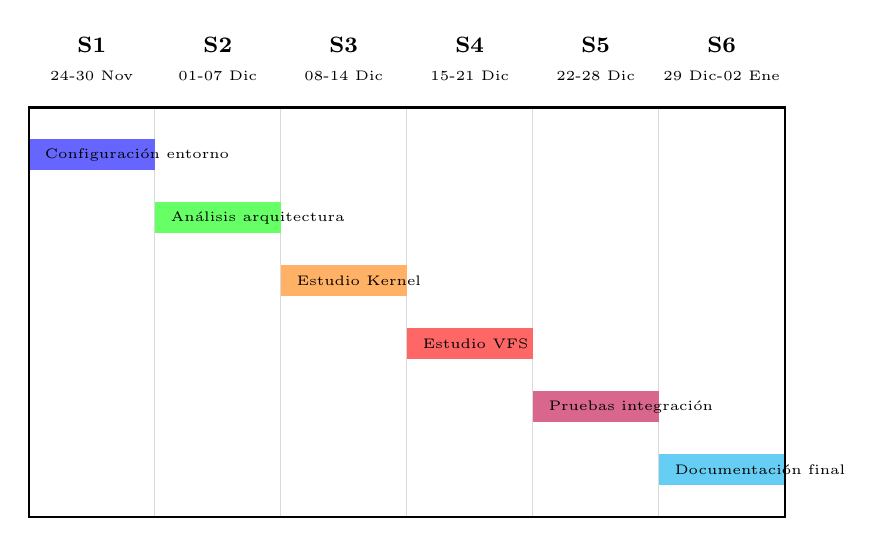
\begin{tikzpicture}[x=0.4cm, y=0.8cm]
    % Encabezados de semanas
    \foreach \i/\fecha in {1/24-30 Nov, 2/01-07 Dic, 3/08-14 Dic, 4/15-21 Dic, 5/22-28 Dic, 6/29 Dic-02 Ene} {
        \node[font=\footnotesize\bfseries] at (\i*4-2, 7.5) {S\i};
        \node[font=\tiny] at (\i*4-2, 7) {\fecha};
    }
    
    % Líneas de separación de semanas
    \foreach \i in {0,4,8,12,16,20,24} {
        \draw[gray!30] (\i, 0) -- (\i, 6.5);
    }
    
    % Actividades (barras)
    % Semana 1: Configuración del entorno
    \fill[blue!60] (0, 5.5) rectangle (4, 6);
    \node[font=\tiny, anchor=west] at (0.2, 5.75) {Configuración entorno};
    
    % Semana 2: Análisis de arquitectura
    \fill[green!60] (4, 4.5) rectangle (8, 5);
    \node[font=\tiny, anchor=west] at (4.2, 4.75) {Análisis arquitectura};
    
    % Semana 3: Estudio del Kernel
    \fill[orange!60] (8, 3.5) rectangle (12, 4);
    \node[font=\tiny, anchor=west] at (8.2, 3.75) {Estudio Kernel};
    
    % Semana 4: Estudio VFS
    \fill[red!60] (12, 2.5) rectangle (16, 3);
    \node[font=\tiny, anchor=west] at (12.2, 2.75) {Estudio VFS};
    
    % Semana 5: Pruebas de integración
    \fill[purple!60] (16, 1.5) rectangle (20, 2);
    \node[font=\tiny, anchor=west] at (16.2, 1.75) {Pruebas integración};
    
    % Semana 6: Documentación final
    \fill[cyan!60] (20, 0.5) rectangle (24, 1);
    \node[font=\tiny, anchor=west] at (20.2, 0.75) {Documentación final};
    
    % Marco
    \draw[thick] (0, 0) rectangle (24, 6.5);
\end{tikzpicture}
\end{center}


\section{Estrategia de pruebas y validación.}

\subsection*{1. Pruebas unitarias}

\begin{itemize}
    \item Funciones pequeñas del kernel (manejo de listas, asignación de estructuras, validaciones internas).
    \item Validación manual y automática mediante logs y assert estructurado.
\end{itemize}

\subsection*{2. Pruebas de integración}

\begin{itemize}
    \item Validación del pipeline completo: arranque del kernel $\rightarrow$ inicialización $\rightarrow$ scheduler $\rightarrow$ VFS $\rightarrow$ CLI.
    \item Empleo de scripts en QEMU para generar escenarios repetibles.
\end{itemize}

\subsection*{3. Pruebas de regresión}

\begin{itemize}
    \item Comparación entre versiones para asegurar que cambios recientes \textbf{no rompen el arranque} ni la CLI.
\end{itemize}

\subsection*{4. Pruebas de experiencia de usuario}

\begin{itemize}
    \item Comandos del shell, manejo de errores, mensajes coherentes, terminación de procesos inválidos.
\end{itemize}

\section{Posibles riesgos y cómo mitigarlos.}

\begin{landscape}
\renewcommand{\arraystretch}{1.35}

\begin{longtable}{|p{3.5cm}|p{5.2cm}|p{1.6cm}|p{2cm}|p{5cm}|p{5cm}|}
\caption{Tabla de riesgos ampliada} \\
\hline
\textbf{Riesgo} &
\textbf{Descripción técnica} &
\textbf{Impacto} &
\textbf{Probabilidad} &
\textbf{Mitigación} &
\textbf{Indicadores tempranos} \\
\hline
\endfirsthead

\hline
\textbf{Riesgo} &
\textbf{Descripción técnica} &
\textbf{Impacto} &
\textbf{Probabilidad} &
\textbf{Mitigación} &
\textbf{Indicadores tempranos} \\
\hline
\endhead

\hline
\multicolumn{6}{r}{Continúa en la siguiente página} \\
\endfoot

\hline
\endlastfoot

Fallas al construir el toolchain &
GCC o Binutils no compilan correctamente para la arquitectura objetivo &
Alto &
Media &
Usar script oficial, verificar dependencias, versiones compatibles &
Errores de linking o binarios incompletos \\
\hline

Kernel panic o page faults &
Punteros nulos, errores en manejo de interrupciones o memoria &
Alto &
Alta &
Validar punteros, usar logs del kernel en cada módulo &
Reinicios inesperados, caída antes del scheduler \\
\hline

Integración inconsistente entre módulos &
Cambios en kernel que afectan procesos o VFS &
Alto &
Media &
Commits pequeños, pruebas continuas, interfaces claras &
Errores en syscalls o creación de procesos \\
\hline

Falta de documentación interna &
Dificultad para comprender estructuras internas del kernel &
Medio &
Alta &
Revisar código fuente, analizar diagramas, revisar tesis y reportes &
Bloqueos del equipo en análisis \\
\hline

Baja performance o deadlocks &
Scheduler inestable o locks mal implementados &
Alto &
Media &
Scheduler simple, no agregar complejidad innecesaria &
Procesos que no terminan o se congelan \\
\hline

Escasez de tiempo del equipo &
Tareas que se extienden más de lo esperado &
Medio &
Media &
Dividir roles, Scrum semanal, priorizar mínimo viable &
Retraso desde semana 2 en adelante \\
\hline

VFS incompleto o inconsistente &
Lectura/escritura fallida o tabla de inodos incorrecta &
Medio &
Media &
Implementación incremental, validar caso mínimo &
Archivos que no montan, errores en CLI \\
\hline

Problemas de compatibilidad en QEMU &
Emulación inconsistente o flags incorrectos &
Bajo &
Media &
Usar parámetros probados, logs seriales &
QEMU se congela o no muestra consola \\
\hline

Sobrecarga en el kernel educativo &
Añadir funciones innecesarias o fuera del alcance &
Medio &
Baja &
Control estricto del alcance (scope) &
Demoras y complejidad excesiva \\
\hline

\end{longtable}
\end{landscape}
